\section{Model Generalization on Other Precipitates}

Finally, it is well known that Mg may contain other phases that can function as cathodic sites in Mg corrosion. Examples are the $\beta$-phase, $Mg_{17}Al_{12}$ \cite{guo2017influence}, Cu \cite{kawabata2012influence} and Ni \cite{hanawalt1942corrosion}. In fact, Song and Artens \cite{song2003understanding} claim that of the three types of second-phase particles that are rich in Ni, Fe and Cu, respectively, Ni is the most detrimental with Fe intermediate to Ni and Cu. Thus, the high-throughput computational strategy was applied to Cu and Ni particles cases by again following the three criteria in Section 2.1 to investigate whether the 6 p-block elements can inhibit HER on surfaces of these second-phase particles. 

\begingroup
\begin{figure}[!ht]
  \centering
  \subfigure[]{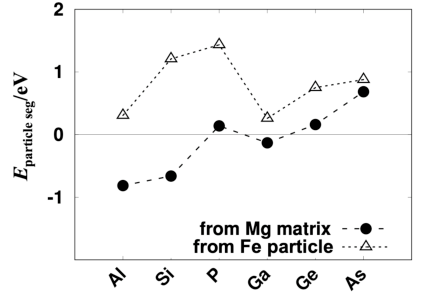
\includegraphics[width=0.49\linewidth]{Chap3/plots/Fig12a.pdf}}\label{Chap:Mg_H:fig:12a}
  \subfigure[]{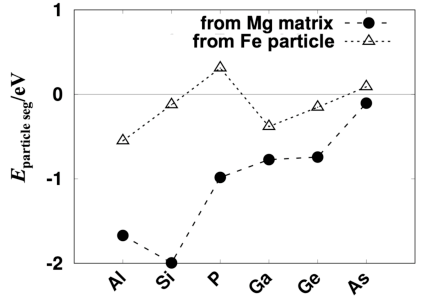
\includegraphics[width=0.49\linewidth]{Chap3/plots/Fig12b.pdf}}\label{Chap:Mg_H:fig:12b}
  \\
  \subfigure[]{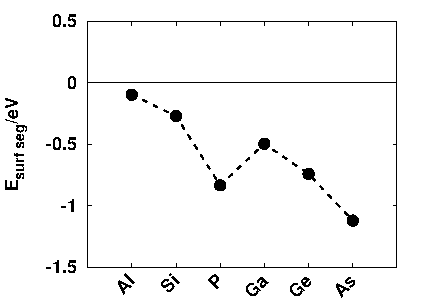
\includegraphics[width=0.49\linewidth]{Chap3/plots/Fig12c.pdf}}\label{Chap:Mg_H:fig:12c}
  \subfigure[]{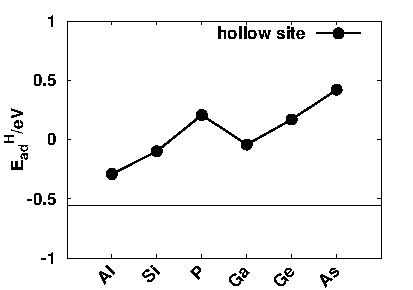
\includegraphics[width=0.49\linewidth]{Chap3/plots/Fig12d.pdf}}\label{Chap:Mg_H:fig:12d}  
\caption[Effects of 6 p-block elements on other precipitates(Cu and Ni)]{(a) and (b): Bulk segregation energies $E_{particle seg}$ for 6 p-block alloying elements in bulk Cu (a) and Ni (b) second-phase particles in Mg matrix, respectively. The solid circles denote the segregation energies of alloying elements in bulk Cu/Ni particles over bulk Mg matrix, and the open triangles denote the segregation energies of alloying elements in bulk Cu/Ni particles over bulk Fe particles. The energy differences are defined in equations similar to Eq. \ref{Chap:Mg_H:eq:particle_seg}. Preference for a bulk Cu/Ni particle over the bulk Mg/Fe particles requires that an alloying element should have a significantly negative value of $E_{particle seg}$. (c) Surface segregation energies $E_{surf seg}$ defined in Eq. \ref{Chap:Mg_H:eq:surf_seg} for Ni (111) of 6 p-block alloying elements. A qualified alloy candidate should have a strongly negative value of Esurf seg. (d) H adsorption energies $E_{ad}^H$, which is defined in Eq. \ref{Chap:Mg_H:eq:H_ads}, on (2x2) Ni (111) surfaces with $\frac{1}{4}$ \ac{ML} alloying atom in the top surface layer. The horizontal line stands for the H adsorption energy of pure Ni (111) surface hollow site.}
  \label{Chap:Mg_H:fig12}
\end{figure}
\endgroup

For the first criterion, we calculated the alloy segregation energy in the bulk of Cu and Ni particles when the alloying element X comes from the Mg matrix or bulk Fe particles via following Eq. \ref{Chap:Mg_H:eq:particle_seg}. For Cu, only Al and Si have a strong energetic preference (more negative than -0.5 eV) to stay in bulk Cu particles compared to bulk Mg as shown by closed black circles in Fig. \ref{Chap:Mg_H:fig12} (a). The segregation energies for P, Ga or Ge are between $\pm$0.1 eV, and As even has a strong segregation (over +0.5eV) in Mg bulk matrix relative to bulk Cu particles.  Therefore, As, Ge, Ga or P does not have a strong preference to be stable in Cu bulk. In addition, all the six p-block elements show thermodynamic preferences for bulk Fe particles over bulk Cu particles as shown by the open triangles in Fig. \ref{Chap:Mg_H:fig12} (a). Alternatively, Fig. \ref{Chap:Mg_H:fig12} (b) suggests that each of the six elements have a thermodynamic preference to stay in bulk Ni particles compared to the bulk Mg matrix, and all of these elements do not show a strong thermodynamic preference for bulk Fe particles over bulk Ni particles. Therefore, the ability of the six p-block alloying elements to inhibit HER on Cu particles is limited and out of the scope of further discussions, and we will only focus on Ni.


For the second criterion, the surface segregation energies of the six elements were calculated via Eq. \ref{Chap:Mg_H:eq:surf_seg}, which shows that all the six elements are also more stable on the clean Ni(111) surface compared to Ni bulk according to Fig. \ref{Chap:Mg_H:fig12} (c). For the calculations of H adsorption energies $E_{ad}^H$, defined in Eq. \ref{Chap:Mg_H:eq:H_ads}, H adsorption energies at the FCC hollow site on Ni(111) surfaces were investigated by only allowing H and surface atoms to relax in the direction normal to the Ni(111) surface, following what was done for Fe (110) as described in Section 3c. Similar to their effects on the surfaces of Fe second-phase particle, all six p-block elements weaken H adsorption energies on Ni (111) surfaces as shown in Fig. \ref{Chap:Mg_H:fig12} (d). On (2x2) pure Ni (111) surfaces, the H adsorption energy is -0.56 eV for $\frac{1}{4}$ ML H coverage. Among the six elements, As, P and Ge alloyed surfaces show very weak H adsorption energies (to +0.42, +0.21 and +0.17 eV, respectively, comparable to $E_{ad}^H$ on the noble metal (Au, Ag) surfaces in Fig. \ref{Chap:Mg_H:fig1} (b)). Germanium, Si, and Al can moderately weaken H adsorption energies (to -0.04, -0.10 and -0.29 eV). Hence, the six p-block elements that are effective on the two Fe surfaces are also effective on Ni(111).